\section{Preliminaries}







\subsection{Problem setup}


We consider the following least squares approximation problem:

\begin{equation}\label{eq:leastsquares}
% \begin{aligned}
    \min_{\bm z} L(\bm z) =  \frac{1}{2} \sum_{j=1}^s |f_{\bm z}(x_j) - y_j|^2
    % &\mbox{ where } \,\,\, f_{\bm z}(x) = \sum_{i=1}^m c_i [a_i x + b_i]_+, \quad \bm z = (\bm a \in \RR^m, \bm b \in \RR^m, \bm c \in \RR^m),
% \end{aligned}
\end{equation}

where $S = \{ (x_i, y_i) \in \RR^2, \, i =1,\ldots, s\}$ is a given set of $s$ samples and $\bm z$ is a vector of \emph{parameters}. Our functional space is the family of 1D feedforward shallow ReLU networks with exactly $m$ neurons. We discuss detailed properties of this space in Section \ref{sec:cpl}. In this paper, we focus on the overparameterized setting $m \gg s$. We will consider several functionally equivalent parameterizations for $f_{\bm z}$ discussed below.

The standard parameterization for $f_{\bm z}$ is

\begin{equation}\label{eq:standard_parameterization}
    f_{\bm z}(x) = \sum_{i=1}^m c_i [a_i x + b_i]_+, \quad \bm z = (\bm a \in \RR^m, \bm b \in \RR^m, \bm c \in \RR^m).
\end{equation}

In the standard parameterization, the knots of $f_{\bm z}$ are the points where the operand inside a ReLU activation changes sign:

\begin{equation}\label{eq:knots}
e_i = -\frac{b_i}{a_i}, \quad a_i \ne 0, \quad i=1,\ldots,m.
\end{equation}

See the left image in Figure~\ref{fig:knots} for an example of a function $f_{\bm z}$ and its knots. 

\begin{figure}
    \centering
    \minipage{0.5\textwidth}
    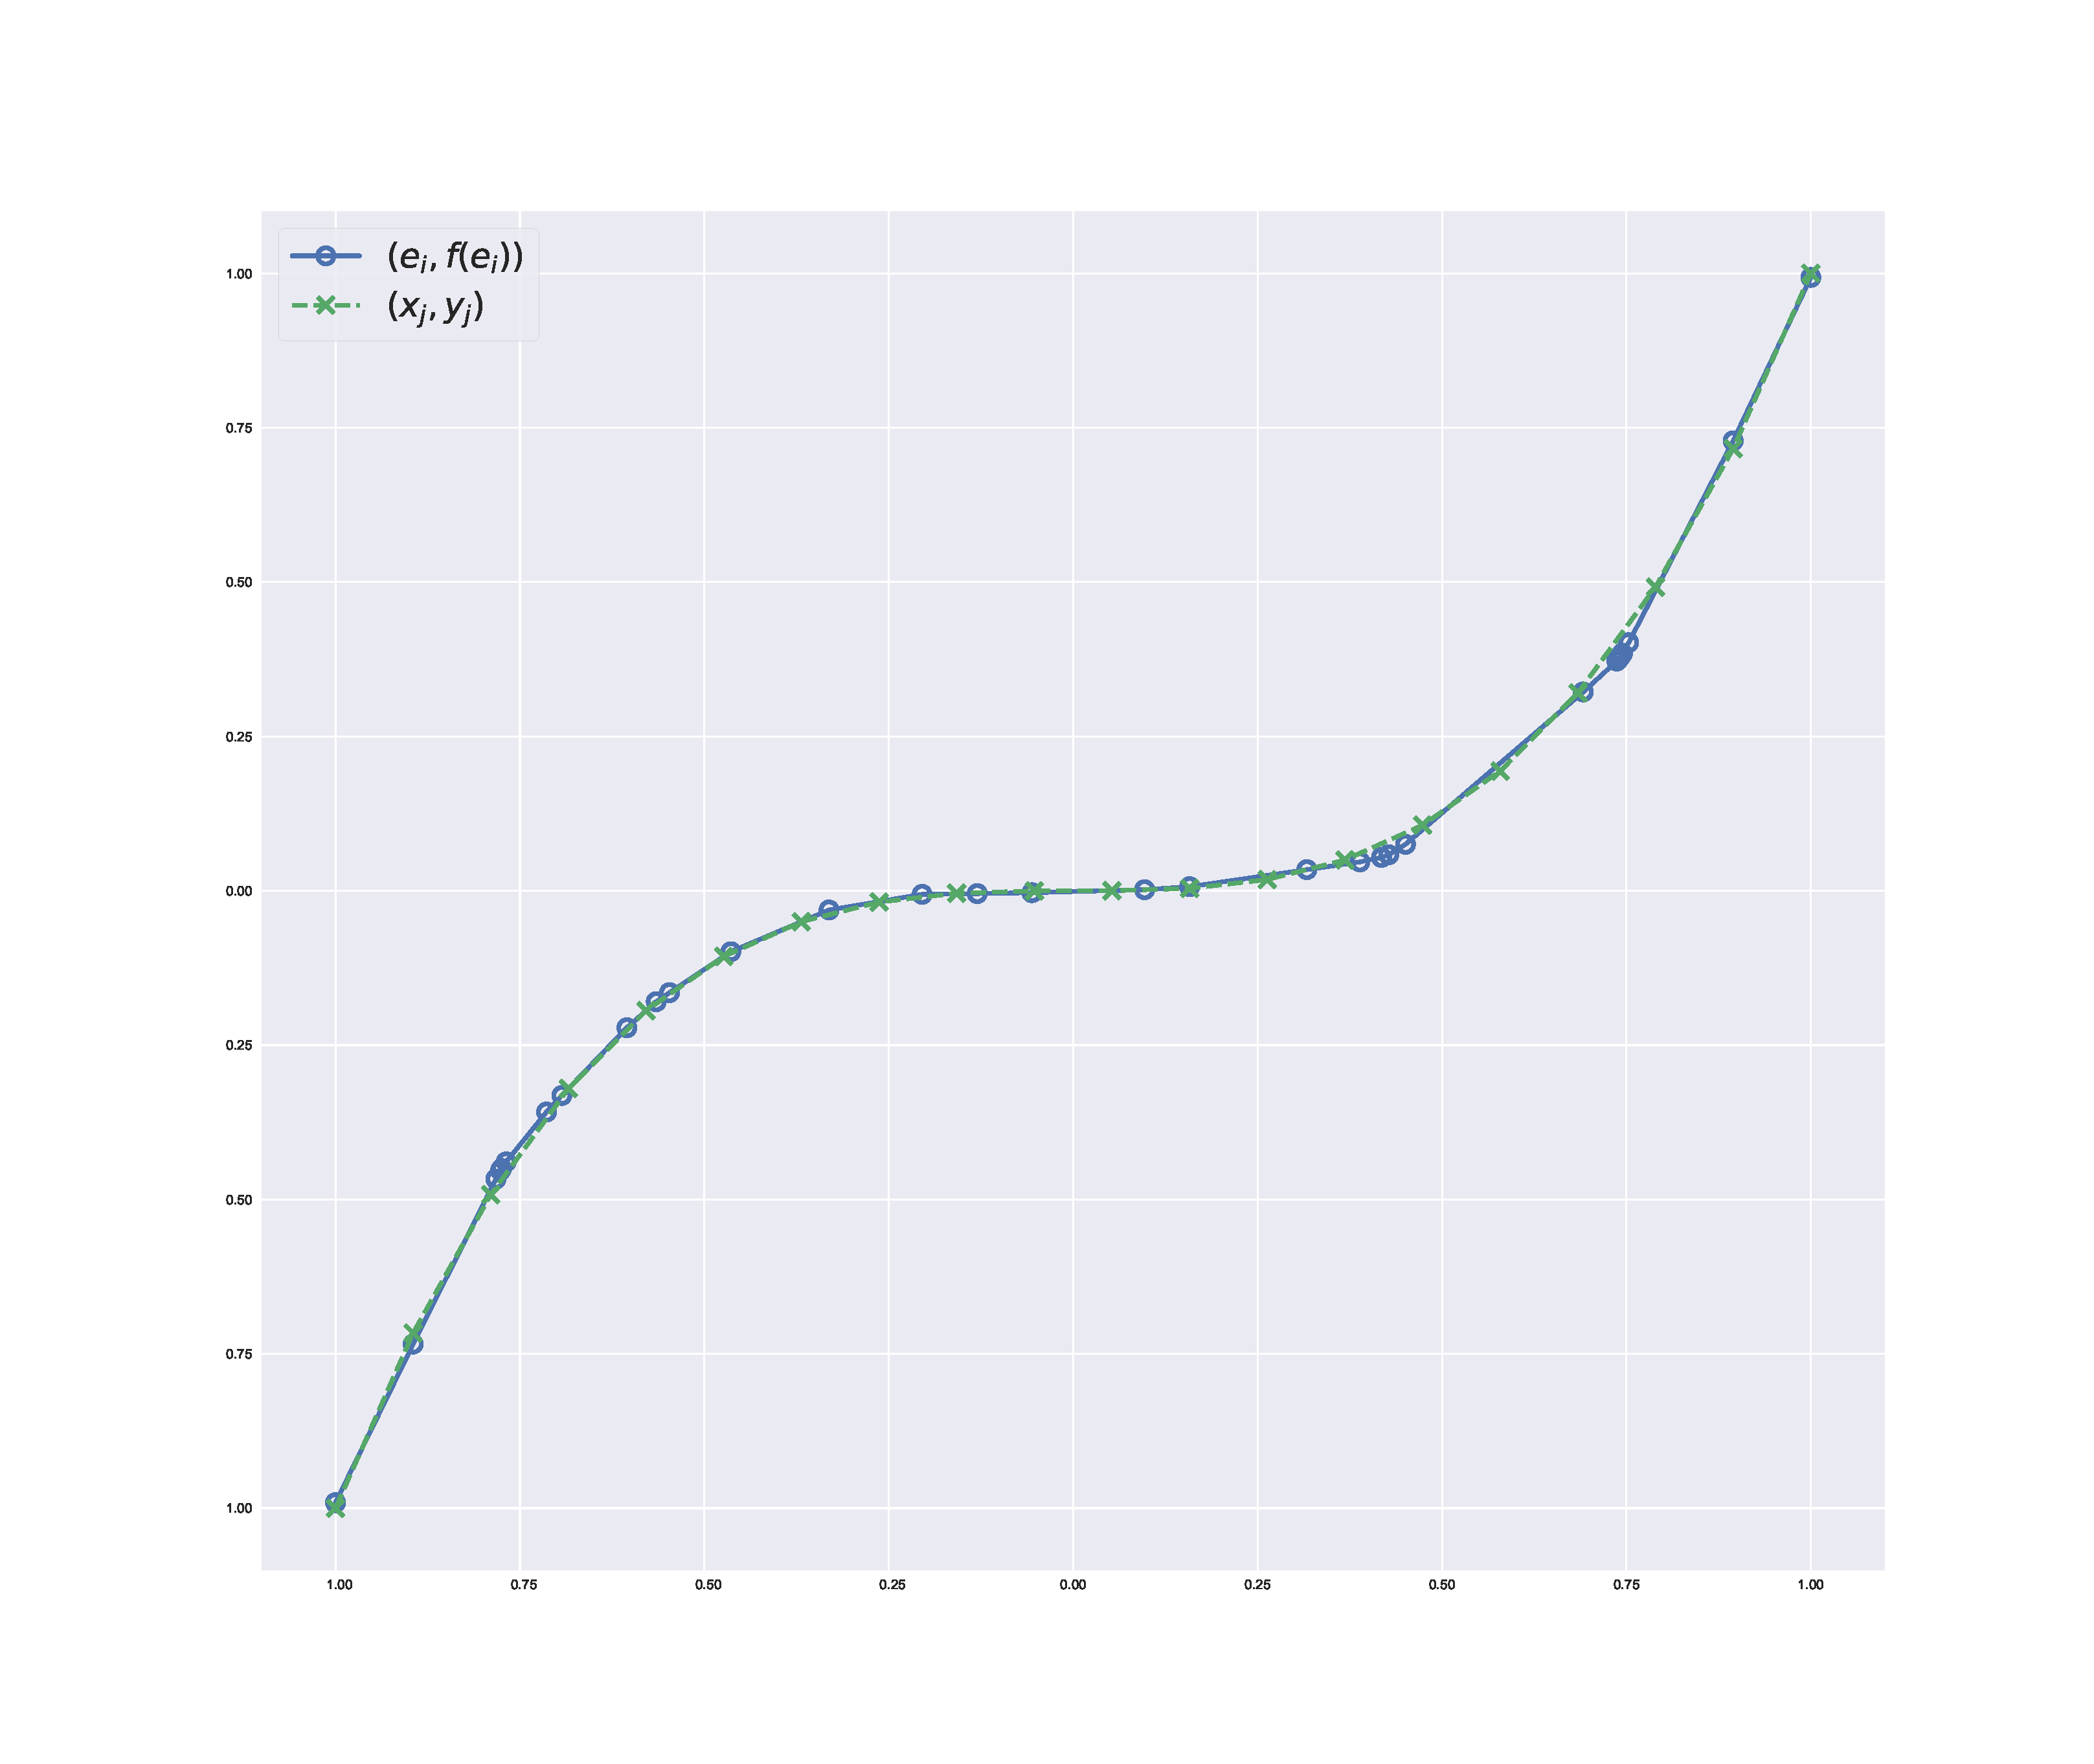
\includegraphics[width=\textwidth]{figures/knots2.pdf}
    \endminipage\hfill
    \minipage{0.5\textwidth}
    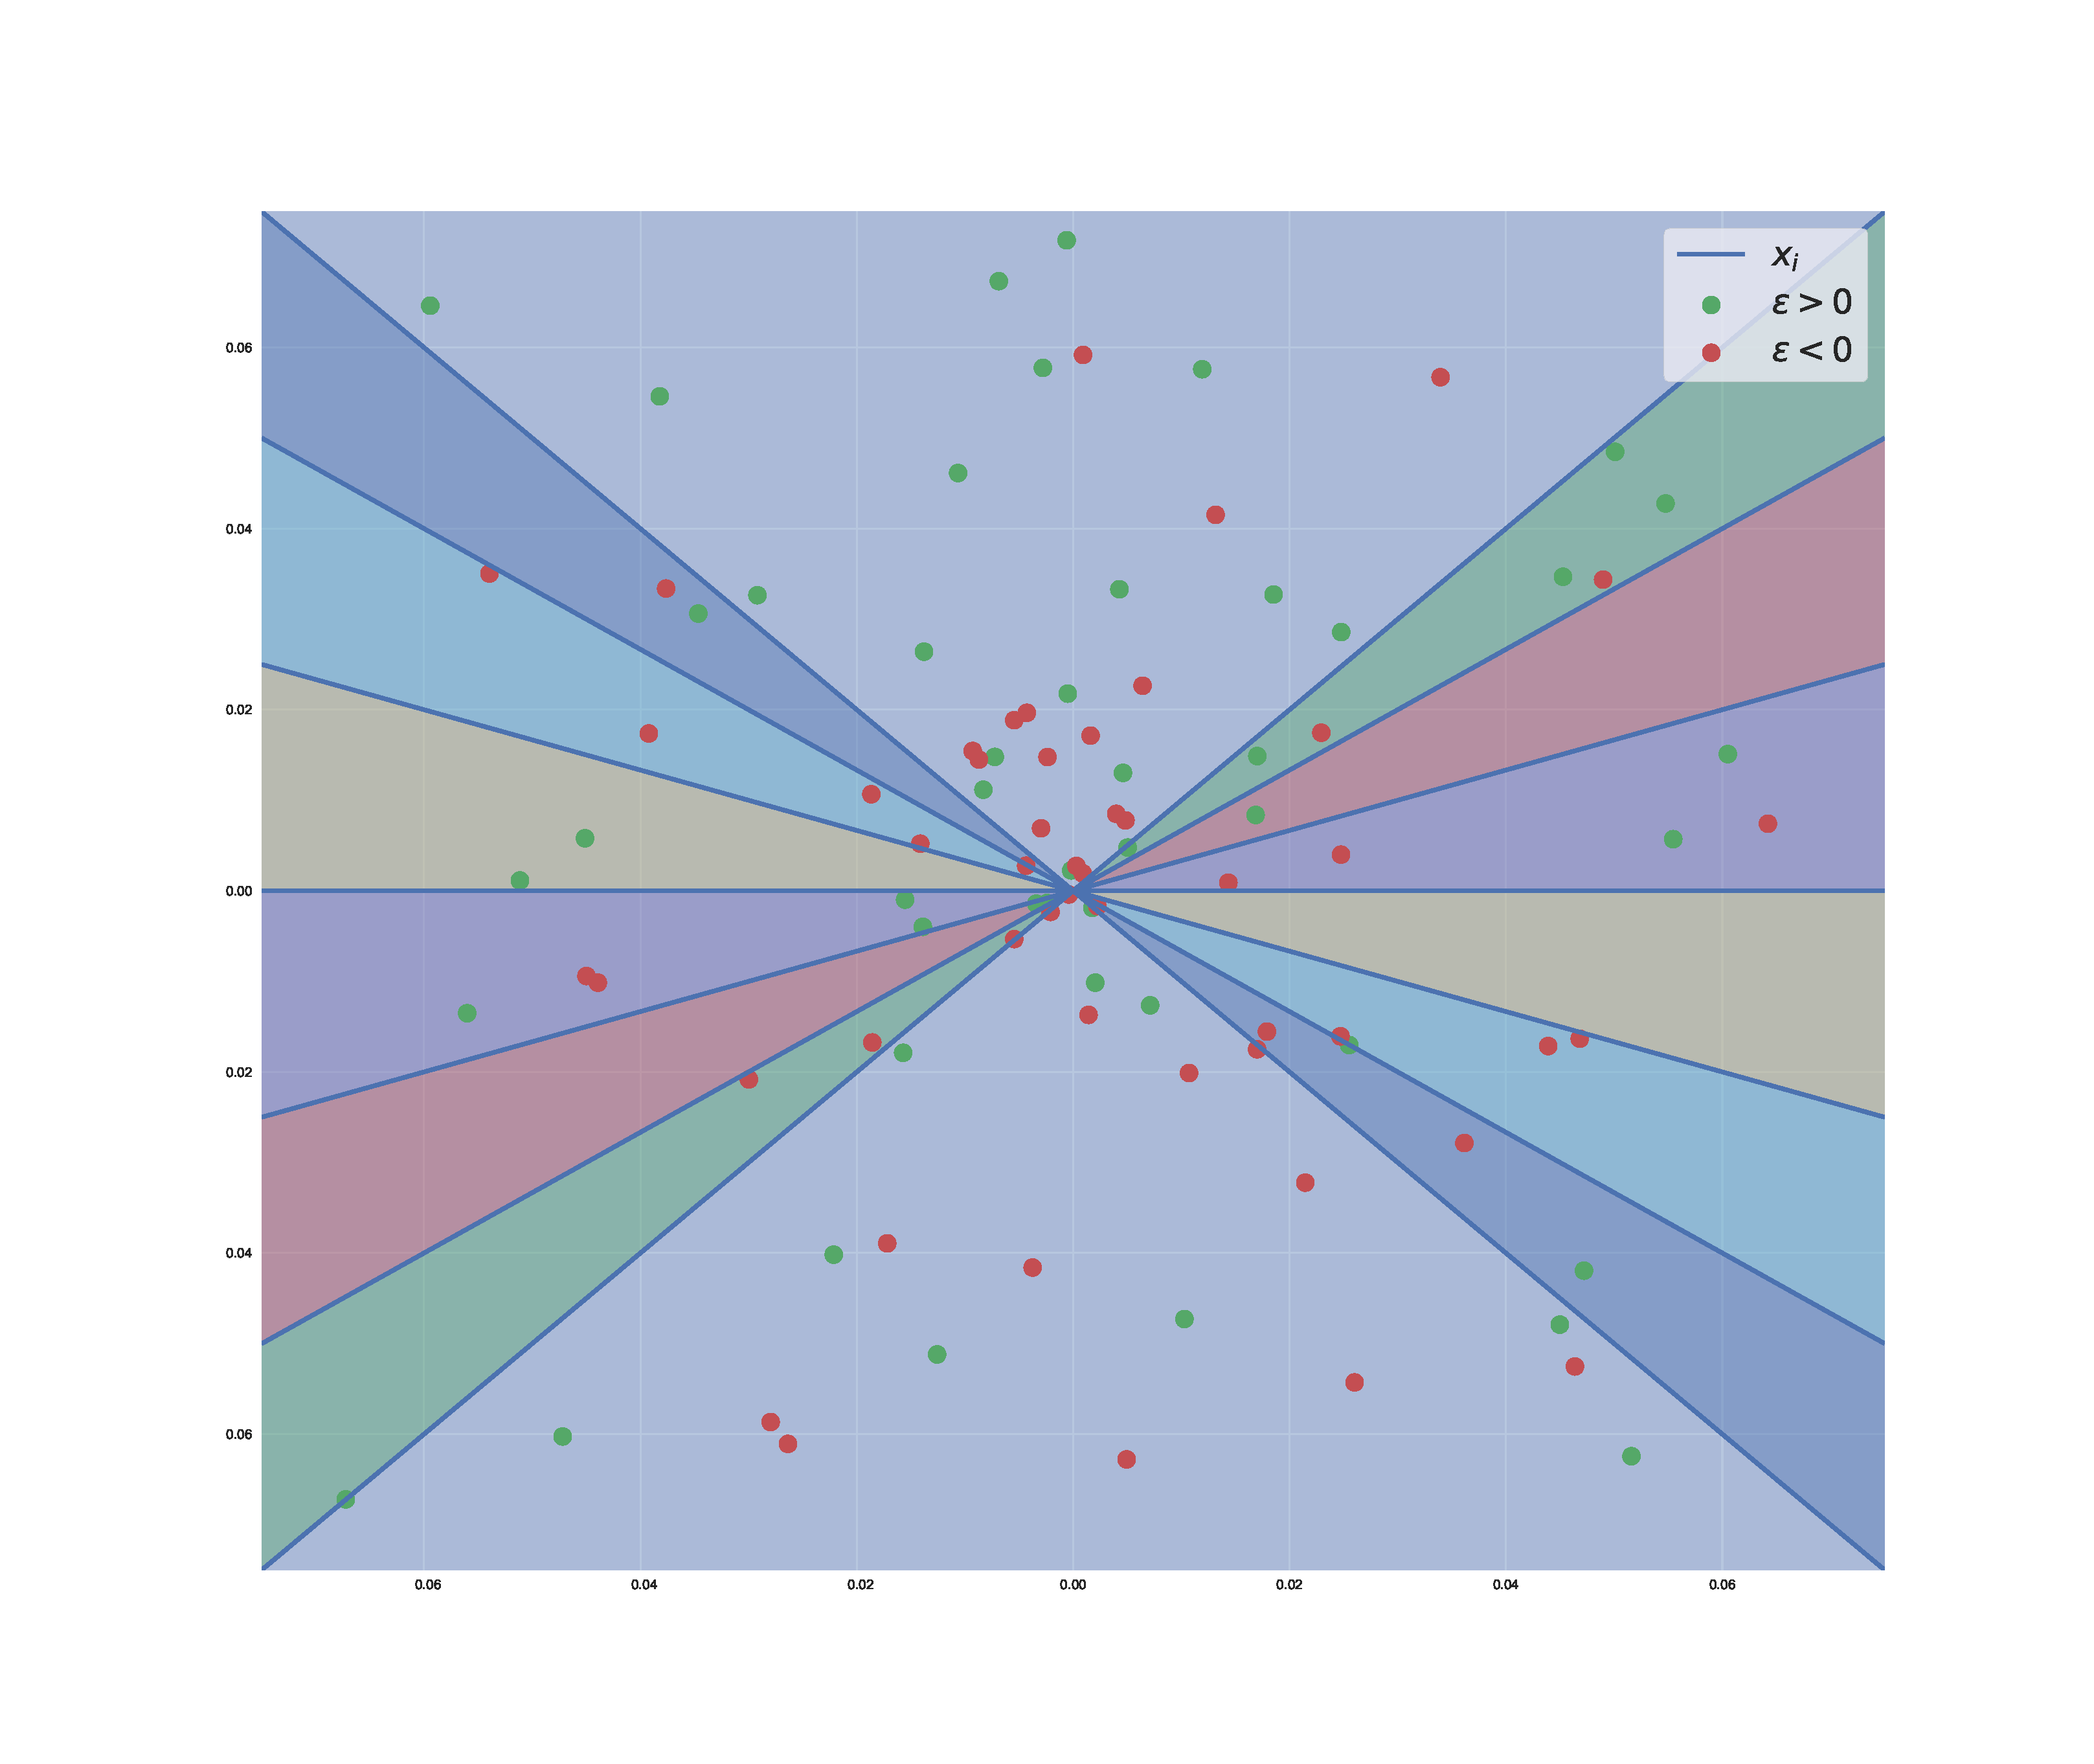
\includegraphics[width=\textwidth]{figures/phaseplot_eg.pdf}
    \endminipage\hfill
    
    
    \caption{\textit{Left:} input samples $(x, y) = (x_j, y_j)_{j=1}^s$ (blue x's) to which we fit a neural network $f_{\bm \xi}(x)$ using the least squares loss \eqref{eq:leastsquares}. $f_{\bm \xi}(x)$ is piecewise linear with the boundaries between pieces occurring at $(e_i, f_{\bm \xi}(e_i))_{i=1}^m$ (green circles). These points correspond to when the operand to one of the ReLUs in \eqref{eq:leastsquares} goes from positive to negative or vice-versa. \textit{Right:} the neurons $\xi_i = (\epsilon_i, u_i, v_i)$ plotted in $u-v$ space. The color of each neuron indicates the sign of $\epsilon_i$. Oberser that the samples $x_j$ correspond to the lines $u x_j + v = 0$ in this space. These sample lines divide the space into the colored regions which correspond to different activation patterns.}
    \label{fig:knots}
\end{figure}



\subsection{Phase Space Parameterization}

A useful parameterization for visualizing the dynamical behavior of a neural network is the \emph{phase space parameterization}

\begin{equation}
    f_{\bm z}(x) = \sum_{i=1}^m \epsilon_i [u_i x + b_i]_+, \quad \bm z = (\bm \epsilon \in \{1, 0, -1\}^m, \bm u \in \RR^m, \bm v \in \RR^m),
\end{equation}.

We can transform from the standard parameterization to the phase parameterization with the map 

\begin{equation}\label{eq:reduced_params}
(\epsilon_i, u_i,v_i) = (\text{sign}(c_i), |c_i|a_i,|c_i| b_i), \qquad i=1,\ldots,m.
\end{equation}

While the standard parameterization \eqref{eq:standard_parameterization} can be used to illustrate the graph of the network function $f_{\bm z}(x)$ at a snapshot in time (Figure~\ref{fig:knots}, left), the phase parameterization gives a more informative view, allowing us to plot each neuron as a 2D particle at position $(u_i,v_i)$, colored depending on the sign $\epsilon_i$ (Figure~\ref{fig:knots}, right), and to visualize trajectories of individual neurons in the plane. 

In the standard parameterization, a neuron $(a_i, b_i, c_i)$ coincides with a point $x$ if $\frac{-b_i}{a_i} = \frac{-v_i}{u_i} = x$. Thus, in phase space, a sample point $x_j$ corresponds to the line satisfying the equation $u x_j + b = 0$. These sample lines, divide the phase space into \emph{activation regions} where a neuron has a fixed \emph{activation pattern} (the colored regions in the right image of Figure~\ref{fig:knots}). These regions correspond to the sets

\begin{equation}\label{eq:activatioon_region}
    R(\bm \tau) = \{ (u, v) \, | \, \text{sign}(u x_j + v) = \tau_j \}, \qquad \bm \tau \in \{1, 0, -1\}^s.
\end{equation}


\subsection{Two Regimes of Gradient Flow}

Our goal is to solve \eqref{eq:leastsquares} using the \emph{gradient flow} (the continuous-time limit of gradient descent) of the least squares loss for a general parameterization of $f_{\bm z}$:

\begin{equation}\label{eq:gradient_flow}
    \bm z(0) = \bm z_0, \qquad \bm z'(t) \in \partial L(\bm z(t)).
\end{equation}

Here $\partial L(\bm z)$ denotes the \emph{Clarke subdifferential}~\cite{clarke1975generalized}, since $L(\bm z)$ is only piecewise smooth. At generic smooth points $\bm z$, the subdifferential coincides with the gradient $\partial L(\bm z(t)) = \{\nabla L(\bm z)$\}. 


% However, we argue in \todo{Section \ref{sec:todo}} that the discontinuities of the gradient play an important role in the dynamics in practice. 

We argue that the gradient flow can be understood by investigating two extreme regimes, corresponding to one of the following dynamics written in the standard parameterization \eqref{eq:standard_parameterization}:

\begin{align}
    (\bm a_0, \bm b_0, \bm c'(t)) & \in -(\,\bm a_0, \bm b_0, \partial_{\bm c} L(\bm z(t))\,)\label{eq:kernel_gf} \\[.3cm]
    (\, \bm a'(t), \bm b'(t), \bm c'(t)) &\in -(\partial_{\bm a} L(\bm z(t)), \partial_{\bm b} L(\bm z(t)), \partial_{\bm c} L(\bm z(t))\, ),\label{eq:adaptive_gf}
\end{align}

Here, \eqref{eq:kernel_gf} corresponds \emph{Kernel Learning}: fixing the inner layer parameters $\bm a, \bm b$ and optimizing over $\bm c$, and \eqref{eq:adaptive_gf} corresponds to \emph{Adaptive Learning}: optimizing over all the parameter $\bm z$. The dynamics of~\eqref{eq:gradient_flow} is a mixture of these two regimes, depending on the initialization of each neuron.

\begin{remark}
As shown in~\cite{NTKJacot}, the dynamics of gradient flow can be expressed in terms of a \emph{tangent kernel}. In particular, the tangent kernel of a two layer network is the sum of two kernels, corresponding to the parameters of each layer. The dynamics of Kernel and Adaptive Learning amount to considering only one of these two kernels.
\end{remark}




